
\documentclass{article}

\usepackage[utf8]{inputenc}
\usepackage[framemethod=tikz]{mdframed}
\usepackage{amsthm, amssymb, amsmath}
\usepackage{listings}
\usepackage[margin=1in]{geometry}
\usepackage{graphicx}
\graphicspath{ {images/} }
\usepackage[demo]{graphicx}
\usepackage{caption}
\usepackage{float}
\usepackage{subcaption}

\title{Non-Adiabatic Explosion}
\author{Kylee Budai\\Shane Sarnac\\Ryan Matthews}
\date{\today}

\begin{document}

\maketitle


\begin{abstract}
    \noindent  Computers are powerful tools. They enable people to connect across networks to locations all over the planet and automate heavy machinery in many manufacturing disciplines. In Mathematics, computers become useful for generating numerical solutions in situations where exact values cannot be derived analytically. This paper aims to apply and investigate the accuracy of important numerical algorithms when estimating solutions for a real world problem: determining if and when a box containing a certain set of reactants will explode. 
\end{abstract}
\section*{Introduction}
 In this investigation, a variety of numerical methods are applied to approximate solutions to a real world problem and evaluated for accuracy based on theoretical outcomes associated with the problem. In particular, this paper investigates properties concerning the Adiabatic Explosion Problem, in which an insulated box filled with potentially combustible materials is analyzed to determine if and when it will explode. To accomplish this task, the fourth order Runge-Kutta method is used to estimate the curve describing the relationship between the temperature inside the box and time. Meanwhile, to support the accuracy of these results, the root finding Bisection method and Simpson's $\frac{1}{3}$ Rule for integration are used to derive estimates for the short term and long term estimates of the solution. As a result of these tests, the numerical methods for approximation are found to be accurate and helpful for deriving interesting information about a real-world problem.  
\section*{Background}
Consider an insulated box with copious amounts of fuel and oxidizer.  The temperature outside of the box is a constant $T_0$ and the initial temperature inside of the box is given by $T(t=0)=T_0$.  The chemical reaction between the fuel and oxidizer will increase the temperature of the box and will either lead to an explosion or a fizzle, depending on certain parameters.  In order to begin to consider the mathematics behind this problem, it is necessary to understand the physical implications.  The conservation of thermal energy within the box is given by $$\frac{dE_{box}}{dt} = \frac{dE_{reaction}}{dt} - \frac{dE_{loss}}{dt}$$ 
which says that the change of energy in the box must be equal to the generation of energy by the reaction minus the energy lost to the environment, a result of the not-necessarily perfect insulation.  Assuming that the fuel concentration ($A_f$) is relatively constant, this conservation of energy equation can be written in terms of temperature.  It becomes $$c_v \frac{dT}{dt} = k_1 \cdot A_f \text{e}^{-E^*/RT} - k_2 \cdot H(T-T_0)$$ where $c_v$ is fixed-volume heat capacity, $k_1, k_2 > 0$ are constants, $E^*$ is the activation energy of the reaction, $R$  is the universal gas constant, and $H$ is the convective heat transfer coefficient.  The first term ($k_1 \cdot A_f \text{e}^{-E^*/RT}$) must be positive to signify a positive heat generation.  Initially, the exponential term is small due to the fact that the activation energy ($E^*$) is much larger than the initial thermal energy of the gas, $RT_0$. Then as the temperature rises, the thermal energy within the box increases, leading to a larger exponential term.  The second term ($ k_2 \cdot H(T-T_0)$)represents heat lost to the environment.  The heat loss must be positive so that subtracting it reduces the energy within the box.  Since the temperature inside of the box will be greater than the temperature outside, $(T-T_0) \geq 0$, and thus $k_2$ must be positive.  \\\\To non-dimesionalize the problem, the following substitutions will be made 
\begin{align*}
    \hat{T} &= \frac{\text{Temperature}}{\text{Initial Temperature}} = \frac{T}{T_0} = 1 + \frac{R\cdot T_0}{E^*}\cdot \theta \quad \text{for some $\theta\in \mathcal{O}(1)$}\\
    \mathcal{T} &= \frac{t}{t_{adiabatic}} 
\end{align*}
where $t_{adiabatic}$ is the explosion time if the insulation were perfect and no heat was lost to the environment. Note that $\frac{R\cdot T_0}{E^*}$, the initial thermal energy of the gas over the activation energy, is much less than 1.  This indicates that $\hat{T}$ is simply 1 plus a small correction, namely $ \frac{R\cdot T_0}{E^*}\cdot \theta$. These substitutions yield the following ordinary differential equation
\begin{align*}
\frac{d\theta}{d\mathcal{T}} &= \text{e}^\theta - \frac{\theta}{\delta}\\
&= \big\{\text{Heat Generation}\big\} - \big\{\text{Heat Loss}\big\}\\
\end{align*}
where $\delta\propto1/H$ is a constant.  Defining $\sigma = \frac{\mathcal{T}}{\delta t_{ref}} $ where $t_{ref}$ is a reference time,  transforms the previous expression to the simple differential equation $$\frac{d\theta}{d\sigma} = \delta \text{e}^\theta-\theta$$ with the initial conditions given by 
\begin{align*}
    \theta(\sigma = 0) &= 0
\end{align*}
Note that $\sigma$ is time scaled by both the adiabatic explosion time and $\delta$ while $\theta$ can be thought of as an non-dimensional representation of heat. 
\subsection*{Explosion vs Fizzle}
The differential equation given above yields two different types of solutions: an explosion or a fizzle.  An explosion will occur where $\frac{d\theta}{d\sigma}>0$ for all $\sigma$ whereas a fizzle will occur when $\frac{d\theta}{d\sigma} \to 0$ as $\sigma \to \infty$.  Thus, solving $$\frac{d\theta}{d\sigma} = \delta^*\text{e}^{\theta} - \theta = 0$$ for $\delta^*$ yields a value of $\delta$ that distinguishes an explosion from a fizzle.  Solving this equation, it is necessary to find the intersection between the functions $y = \theta$ and $y = \delta^* \text{e}^{\theta}$.  Plotting these two functions, it is clear that, at some $\theta^*$, not only are the function values equal but so are the derivatives.  This results the following system 
\begin{align*}
    \delta^* \cdot \text{e}^{\theta^*} &= \theta^*\\
    \delta^* \cdot \text{e}^{\theta^*} &= 1
\end{align*}
which gives that $\theta^* = 1$ and $\delta^* = 1/\text{e}$.  Looking at the magnitude of the derivative for $\delta > \delta^*$ and $\delta < \delta^*$, it is not difficult to conclude that for $\delta > 1/\text{e}$ there will be an explosion and for $\delta<1/e$ there will be a fizzle.\\

\noindent Prior to solving anything numerically, it is important to analytically determine early and late time approximations for cases of both a fizzle and of an explosion.  
\subsubsection*{Explosion and Fizzle (short-time approximation)}
At the start of the reaction, the ordinary differential equation can be approximated by using the fact that $\text{e}^\theta \approx 1+\theta$ for small $\theta$ (Note that this is just a linearization centered at zero).  This approximation reduces the differential equation to
\begin{align*}
    \frac{d\theta}{d\sigma}
                            \approx \delta (1+\theta) - \theta = \delta + \theta(\delta - 1)
\end{align*}
which is solvable analytically and yields the solution
$$\text{ln}\Big(\theta+\frac{\delta}{\delta-1}\Big) = (\delta - 1) \sigma + C$$ where the value of $C$ can be found using the initial condition $\theta(\sigma = 0) = 0$.  After plugging in the initial condition and solving for the constant, this early-time approximation results in
$$\theta \approx \Big(\frac{\delta}{\delta - 1}\Big)\Big[\text{e}^{(\delta-1)\sigma}-1\Big]$$
Note that no assumptions were made to limit this approximation to the explosion or the fizzle so it holds in both cases.

\subsubsection*{Fizzle (long-time approximation)}
To derive an equation for the long term approximation for a fizzle inside the box, the long term behavior of the reaction must be considered. Since $\theta$ represents a non-dimensionalized version of the temperature inside the box, the differential equation 
\begin{align*}
    \frac{d\theta}{d\sigma} = \delta \text{e}^\theta - \theta
\end{align*}
represents the effects of the temperature of the box over a change in $\sigma$, the non-dimensionalized version of time. For an explosion, it would be expected that at some point in time, the change in temperature would increase rapidly and eventually taper off when the amount of substance needed for the reaction runs out. For a fizzling reaction, however, the temperature would be expected to rise near the beginning of the reaction, then gradually taper off and approach a constant value. This suggests that the rate of temperature change after a long period of time will approach zero, indicating that the temperature this kind of reaction approaches can be determined by finding a $\theta_\text{fizzle}$ value that of $\theta$ makes $\frac{d\theta}{d\sigma} = 0$. Using this, $\theta_\text{fizzle}$ can be expressed by the following expression: 

\begin{align*}
   \frac{\text{e}^{\theta_{fizzle}}}{\theta_{fizzle}} = \frac{1}{\delta} 
\end{align*}

\noindent While this expression may be impossible to solve without advanced analytical methods, the solution can be reliably estimated using root finding algorithms like Newton's Method or Bisection. In doing this, the long term behavior of the fizzling reaction can be easily determined for any $\delta < 1/\text{e}$. 

\subsubsection*{Explosion (long-time approximation)}
Unlike the fizzling reaction, an explosion will occur in the box when the change of temperature approaches infinity as time approaches the time of explosion, $t_\text{explosion}$. In terms of the model, $\sigma$ represents time, so as $\sigma$ approaches some $\sigma_{explosion}$, $d\theta/d\sigma$ approaches infinity. 
This sudden increase results in a failure of numerical methods like the Runga Kutta algorithm due to over-stepping beyond $\sigma_\text{explosion}$.  To usefully apply numerical methods to the problem, consider $d\sigma/d\theta$ as opposed to $d\theta/d\sigma$.  This change turns the graph on its side and transforms the vertical asymptote into a horizontal one (since $d\sigma/d\theta \to 0$ as $d\theta/d\sigma\to\infty$). The differential equation then takes the form 
\begin{align*}
    \frac{d\sigma}{d\theta} = \frac{1}{\delta \text{e}^\theta - \theta}
\end{align*}
with initial condition $\sigma(\theta = 0) = 0$.  Now, instead of finding the non-dimensionalized version of temperature that the reaction approaches over the non-dimensionalized version of time, the roles are reversed, finding $\sigma_{explosion}$, the "time"of the explosion. Since $\frac{d\sigma}{d\theta}$ is defined only in terms of $\theta$, the value for $\sigma_\text{explosion}$ can be determined by integrating the expression $$\sigma_{explosion} = \int_0^\infty \frac{d\theta}{\delta \text{e}^\theta - \theta}$$ over all $\theta$. However, this integral is difficult - if not impossible - to solve analytically. As a result, the value of $\sigma_\text{explosion}$ can be approximated by numerically integrating the expression using methods like Simpson's ${\frac{1}{3}}^\text{rd}$ Rule over a well-chosen finite domain. Once $\sigma_{explosion}$ is known, the long-time solution for an exploding reaction is approximated by $$\sigma\approx \sigma_{explosion} - \frac{1}{\delta\text{e}^{\theta}}$$

\section*{Applications}
This section will consider an example of a fizzle and an explosion and will compare the short and long-time solutions to the numerical approximations.
\subsection*{Fizzle}
First consider an example of fizzle by setting $\delta = 1/3$.  This yields the differential equation given by:
$$\frac{d\theta}{d\sigma} = \frac{1}{3}\text{e}^\theta - \theta\\$$
with the initial condition that $\theta(\sigma = 0) = 0$.  As explained above, there is a short-time and long-time approximation to $\theta$, both derived directly from the ordinary differential equation in addition to the physical implications of the problem.  In order to determine the value of $\theta_{fizzle}$, the horizontal asymptote representing the non-dimensionalized version of the temperature the fizzling reaction approaches, a solution for $\theta_{fizzle}$ must be determined from the expression $\frac{\text{e}^{\theta_{fizzle}}}{\theta_{fizzle}} = \frac{1}{\delta}$. Since $\delta = \frac{1}{3}$, this expression becomes $$\frac{\text{e}^{\theta_{fizzle}}}{\theta_{fizzle}} = 3 $$ which corresponds to $d\theta/d\sigma = 0$.  Using bisection with a tolerance of .0001 to solve this equation yields two solutions:
\begin{equation*}
    \theta_{fizzle_1} = 0.619061  \quad  \quad \theta_{fizzle_2} = 1.512134
\end{equation*}
To determine which value of $\theta_{fizzle}$ that the reaction is expected to approach, it is helpful to look at the vector field of $d\theta/d\sigma$ shown below where the orange line represents $\theta_{fizzle_1}$ and the blue line represents $\theta_{fizzle_2}$.
\begin{center}
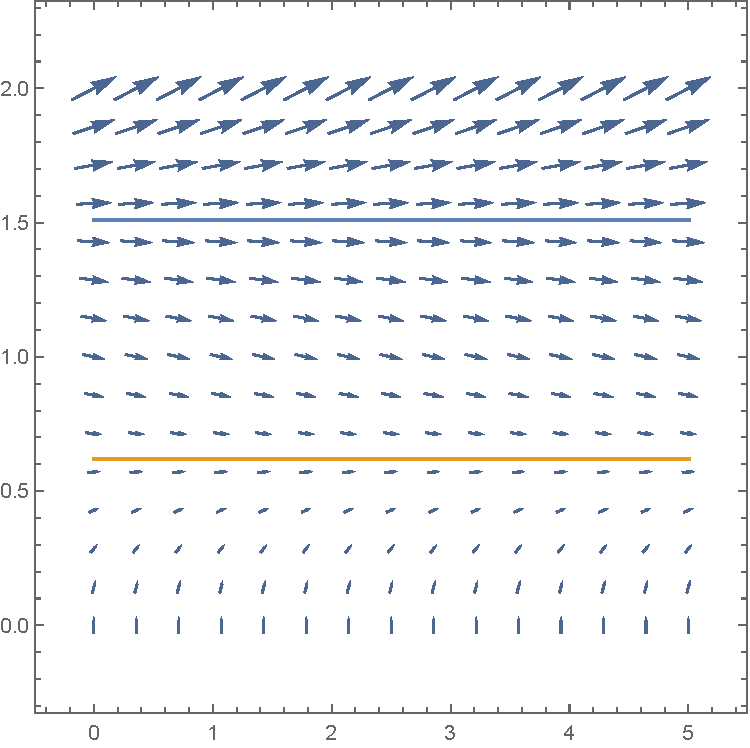
\includegraphics[scale = .3]{vfield}
\end{center}
This vector field shows that $\theta_{fizzle_1}$ is a stable equilibrium while $\theta_{fizzle_2}$ is unstable.  Therefore, $\theta_{fizzle} = \theta_{fizzle_1}$ and the solution of the initial value problem will tend toward $0.619061$ in the long run. This result is also supported by the known initial condition, $\theta(\sigma = 0) = 0$, which, based on the vector plot, would show that the solution will approach $\theta_fizzle_1$. Additionally, in order to keep this problem well-posed, this initial condition cannot be changed, thus the unstable solution represented by $\theta_fizzle_2$ can be disregarded in all future analysis in this example. \\

\noindent Meanwhile, the short term solution (expected to only be valid for $\sigma << 1$) is given by 
\begin{align*}
    \theta &\approx (\frac{\delta}{\delta - 1})(\text{e}^{(\delta - 1)\sigma} - 1) \\
    \theta &\approx -\frac{1}{2}(\text{e}^{-\frac{2}{3}\sigma} -1) \\
    \theta &\approx \frac{1}{2} - \frac{1}{2}\text{e}^{-\frac{2}{3}\sigma}
\end{align*}
as was derived above.\\
\noindent From the given differential equation $\frac{d\theta}{d\sigma} = \delta \text{e}^\theta - \theta$, the full curve representing the relationship between temperature and time can be estimated using the fourth order Runge-Kutta method with a step size of 0.01. The early and late approximations of the solution can be used to check the resulting approximation for accuracy, which is shown in the following figure. 
 
\begin{figure}[H]
\begin{center}
\begin{subfigure}{.5\textwidth}
  \centering
  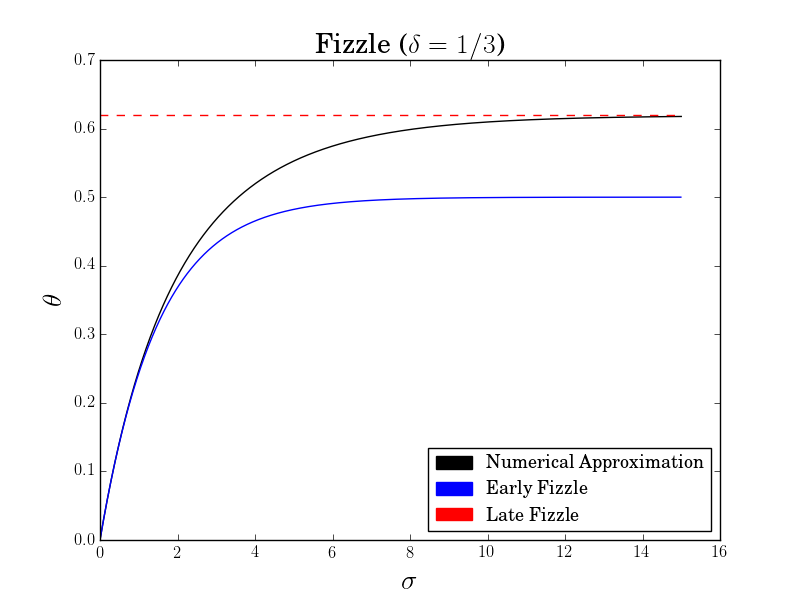
\includegraphics[scale = .4]{fizzle}
  \caption{Full-Domain}
\end{subfigure}%
\begin{subfigure}{.5\textwidth}
  \centering
  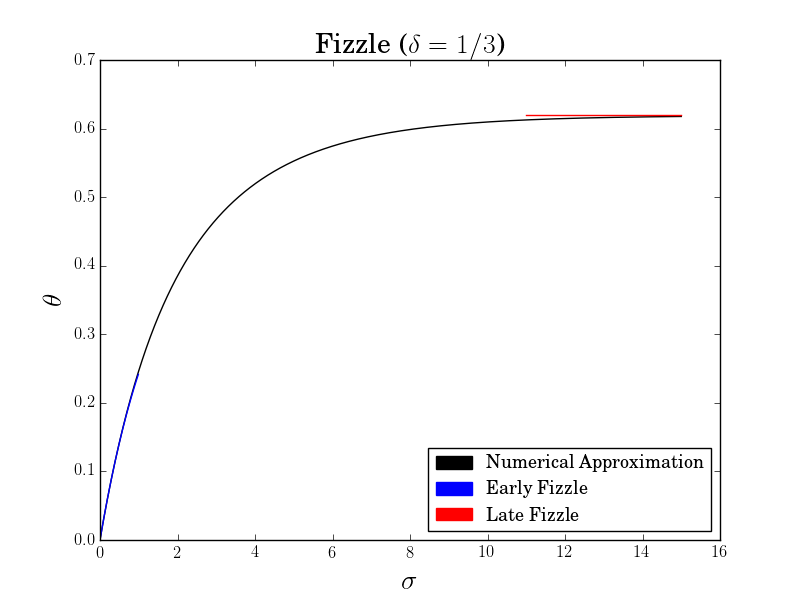
\includegraphics[scale = .4]{fizzleapprox}
  %\caption{A subfigure}
  \caption{Highlighting Approximation Accuracy}
\end{subfigure}
\caption{Early and Late Approximations to Numerical Solution}
\label{fig:test}
\end{center}
\end{figure}
\noindent These plots show the early (short-time) and late (long-time) approximations for the fizzle in addition to the numerical solution to the ordinary differential equation. The purpose of the Full-Domain Plot is to highlight the domain of accuracy of the short and long term solutions by showing the errors of the both approximations in the full domain.  Seeing the information laid out like this is useful in that it is easy to see where it is appropriate to stop plotting the approximations.  Limiting the domain of both the early and late solutions yields plot (b).  It is clear that the early and late solutions provide an accurate fit to the numerical approximation where they are expected to.  In particular, the early solution seems to be a good fit for values of $\sigma$ less than 1 while the late solution provides a good fit for $\sigma > 12$.   Consider if the approximations were not truncated in their appropriate domain and were instead considered full approximations.  The largest error for the late-time solution is at $\theta = \sigma = 0$ and is given by $\theta_{fizzle}$ while the largest error of the short term solution is at the end of the plot and is approximately .15.  It would be easy to misinterpret this finding and say that the early-time approximation is a sufficient estimate for the entire problem because of how seemingly small the error is (of order .1).  This is not the case because of the fact that $\theta$ and $\sigma$ are non-dimensionalized representations of heat and time respectively.  This implies that a seemingly small change in $\theta$ may correspond to a much larger change in temperature and the significance of that change is unclear by merely looking at these plots.\\\newline Looking at the axes of the plots, it is clear that $\theta$, which is a dimensionless representation of temperature, increases very slowly with $\sigma$, the dimensionless representation of time.  In other words, for $\delta = 1/3$, the temperature in the box does not increase quickly enough to lead to an explosion and instead leads to a fizzle. 

\subsection*{Explosion}
Now consider an example of an explosion by setting $\delta = 1$.
Recall that an explosion occurs when $\delta > \frac{1}{\text{e}}$.  To find the time of the explosion, represented by $\sigma_{explosion}$, recall that an explosion occurs where $d\theta/d\sigma$ approaches infinity.  Since it is difficult to catch a drastic increase in slope as was previously discussed, we will consider $d\sigma/d\theta$ which will tend towards zero as opposed to infinity.  Thus, the ordinary differential equation becomes: 
\begin{align*}
    \frac{d\sigma}{d\theta} = \frac{1}{\text{e}^\theta - \theta }
\end{align*}
subject to the initial condition $\sigma(\theta = 0) = 0$.
$\lim_{\theta\to\infty}= 0$ implies that 
\begin{align*}
    \sigma_{explosion} = \int_{0}^{\infty} \frac{1}{\text{e}^\theta - \theta} d\theta
\end{align*}
It is important to notice that despite the fact that the upper bound on the integral is infinity, a finite upper bound will be able to sufficiently approximate the integral because the integrand decreases so rapidly.  Experimentation with different values led to the conclusion that
$$\sigma_{explosion} \approx \int_{0}^{15}\frac{1}{\text{e}^\theta - \theta} d\theta$$
Integrating this expression using Simpson's $\frac{1}{3}$ Rule and a step size of .01 results in an explosion occurring when $\sigma \approx 1.359097$.  Just as with the fizzle, this is a horizontal asymptote for the plot of $\sigma$ as a function of $\theta$.  Switching axes results in it being a vertical asymptote for $\theta$ as a function of $\sigma$, as expected.  Thus, the long-term solution to this problem is given by
$$\sigma\approx 1.359097-\frac{1}{\text{e}^\theta}$$
The short term, valid only for small $\sigma$, solution can be found by plugging $\delta$ into the equation 
\begin{align*}
\theta \approx \frac{\delta}{\delta -1}[\text{e}^{(\delta -1)\sigma} -1]
\end{align*}
Since $\delta = 1$ results in an indeterminate, determining a short-time solution relies on taking a limit as follows
\begin{align*}
    \theta &\approx \lim_{\delta\to1}\Big(\frac{\delta}{\delta - 1}\Big)\Big[\text{e}^{(\delta-1)\sigma}-1\Big]\\
        &= \lim_{\delta\to1}\frac{\text{e}^{(\delta-1)\sigma}-1+ \delta\cdot\sigma \text{e}^{(\delta-1)\sigma}}{1} \quad \text{by L'Hopital's rule}\\
        &= \sigma
\end{align*}
Thus, for small values of $\sigma$, $\theta\approx\sigma$.  

The plots below were generated by applying the fourth order Runge-Kutta method to the ordinary differential equation $(d\sigma/d\theta = 1/(\text{e}^{\theta}-\theta))$ with a step size of .01.  The early and late approximations are also shown on the plot (plotted both for the entire domain and truncated to account for accurate approximation).  It is important to recall that the solution generated is the solution to $d\sigma/d\theta$ but the desired solution was for $d\theta/d\sigma$.  A simple change in axes can be made to account for this initial switch in variables and does not change the numerical results.  
\begin{figure}[H]
\begin{center}
\begin{subfigure}{.5\textwidth}
  \centering
  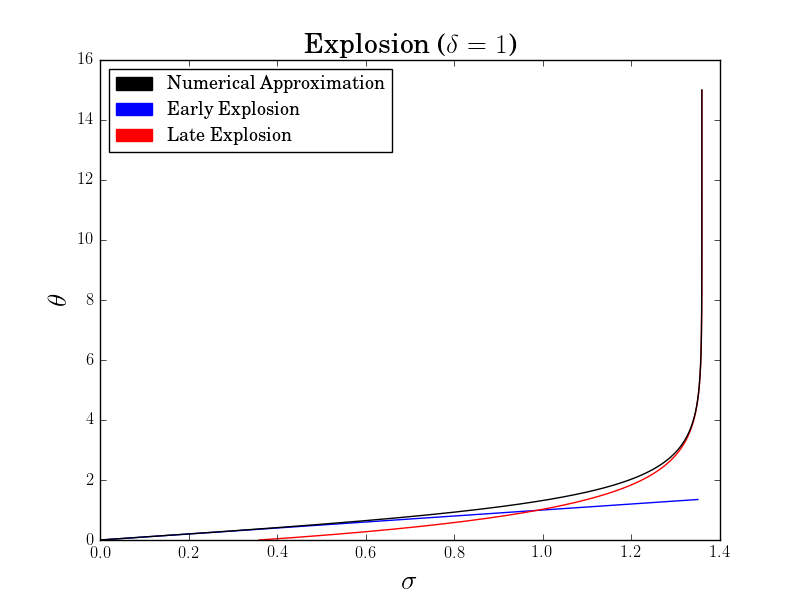
\includegraphics[scale = .4]{explosion}
  \caption{Full Domain}
  \label{fig:sub1}
\end{subfigure}%
\begin{subfigure}{.5\textwidth}
  \centering
  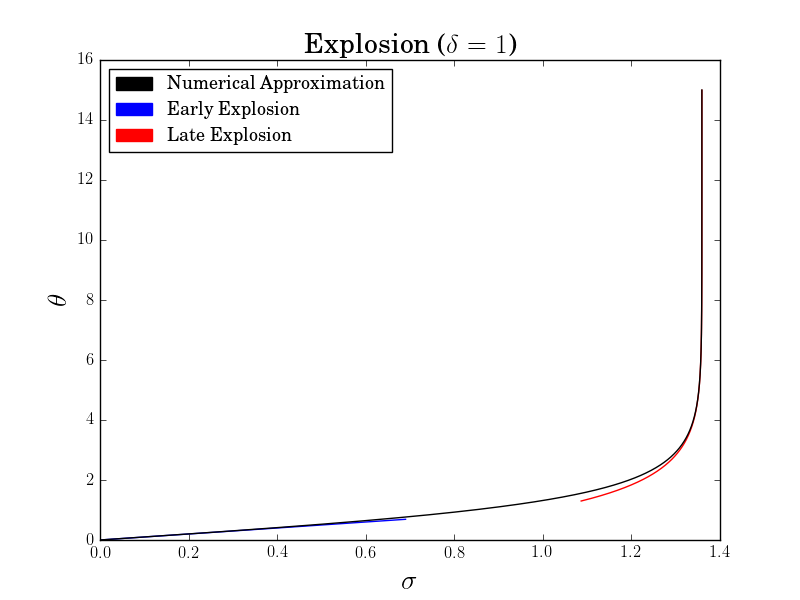
\includegraphics[scale = .4]{expapprox}
  \caption{Highlighting Approximation Accuracy}
  \label{fig:sub2}
\end{subfigure}
\caption{Early and Late Approximations with Numerical Solution}
\label{fig:test}
\end{center}
\end{figure}
Similarly to the fizzle example, the full domain of the late and early approximations are shown to highlight the error of those approximations to the numerical solution.  Plot (b) was generated by recognizing a domain of accuracy on both of the approximations (early and late).  As is shown, the early approximation is accurate for $\sigma<.7$ and the late approximation for $\sigma > 1.2$.  This leaves a domain $.7<\sigma<1.2$ where a numerical approximation is necessary.  Looking at the axes of the plots to determine the largest error of the early and late approximations gives much different results than in the case of the fizzle.  A seemingly small error (when the approximations look very close the the solution) corresponds to a larger error than appears.  An example of this is to look at the intersection of the early and late solutions.  The distance of that point from the numerical solution is approximately .5 which is a huge error considering the fact that the largest error in the fizzle case was around .6.

Looking again at the axes of the plots, and recalling that $\theta$ and $\sigma$ are non-dimensionalized representations of temperature and time respectively, it is clear that as $\sigma$ increases, the value of $\theta$ increases much more drastically.  This corresponds to a rapid increase of the temperature within the box which ultimately leads to an explosion.  

\subsection*{Comparing Results}
As was previously mentioned, looking at the axes on the plots, it is clear that $\theta$ increases much more rapidly as a function of $\sigma$ in the case of an explosion.  This is to be expected because of the fact that a fizzle occurs if the temperature does not increase quickly enough and eventually levels out whereas an explosion corresponds to a sudden increase in temperature that results in a seemingly infinite slope.

As a further comparison between the explosion and fizzle cases, consider the values of each numerical approximation when $\sigma = 1$.  For the fizzle, $\theta(\sigma=1)\approx.58$ whereas for the explosion, $\theta(\sigma=1)\approx 1.5$.   To understand the implications of this, recall how $\theta$ relates to temperature. 
\begin{align*}
    \hat{T} =  \frac{T}{T_0} &= 1 + \frac{R\cdot T_0}{E^*}\cdot \theta \\
    T & = T_0 + \frac{R\cdot T_0^2}{E^*} \theta
\end{align*}  Despite the fact that $\theta$ does not have dimensions, it does have a linear relationship with the temperature in the box.  Therefore, at $\sigma = 1$, the temperature inside the box has increased by approximately three time more in the case of the explosion than in the case of the fizzle.  Noting this drastically larger increase, it is not difficult to intuitively understand why $\delta = 1$ led to an explosion whereas $\delta = 1/3$ did not.  

\section*{Conclusion}
By using numerical methods to solve problems related to the Non-Adiabatic Explosion scenario, we showed that numerical methods can prove to be very useful in certain ranges where analytical solutions are not possible. With this in mind, it is easy to see where these methods could be used in many other real-world scenarios to solve important problems. However, we also showed that numerical computations alone cannot entirely solve a problem. This investigation demonstrated that a lot of ground-work must be done in order to prepare a problem to be solved by computers. As a result, this paper also highlighted the importance of collaboration across disciplines to solve problems, because without the efforts of so many highly trained chemical engineers and mathematicians, we would never know how long it would take for a box to explode (or not). 
\end{document}
